




\chapter{Viewing Options}
\minitoc  

\section{General colour and lightning options}

The general options window contains the following
sections:\\\\
\noindent
\begin{minipage}{0.55\textwidth}
\subsection{Windows}
These controls affect the default colour of objects opened within ISE-MeshTools, the colour of grid elements, and the background colour.
\subsection{Light}
These controls affect the orientation of the light and specular, diffuse and ambient light parameters. By default surface back faces are not shown. Back face lighting can be enabled if the checkbox ``enable two sided lighting" is checked

\end{minipage}  
 \begin{minipage}{0.45\textwidth}\centering
  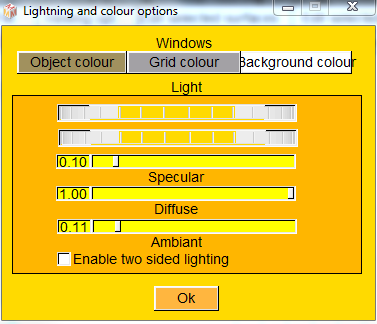
\includegraphics[scale=0.4]{images/Viewing_options/General_colour.png}
 \captionof{figure}{Lightning and colour options window}
 \end{minipage} 
\noindent






\section{General rendering options}
The rendering options window contains the following sections:\\\\


\noindent
\begin{minipage}{0.55\textwidth}
\subsection{Object rendering when moving object/camera}
\underline{Show full surface / scalars (slower):}  when active, surfaces are fully drawn when moving the object or the camera. This results in a better perception of object / camera
movements. This option is convenient when working with light surfaces.\\

\noindent
\underline{Show point cloud (faster)}: 3D surface rendering can be slow using the preceding option when working with:\\
- large number of surfaces simultaneously\\
- heavy surfaces (large number of triangle / vertices)\\

\end{minipage}  
 \begin{minipage}{0.45\textwidth}\centering
  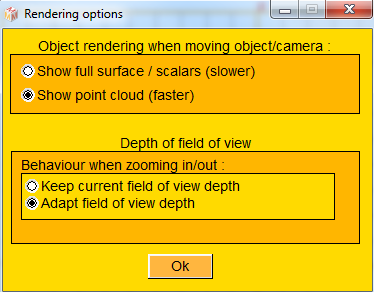
\includegraphics[scale=0.4]{images/Viewing_options/Rendering_options.png}
 \captionof{figure}{Rendering options window}

 \end{minipage} 
\noindent
Also, rendering is slower when tag rendering mode is active (
\includegraphics[scale=0.7]{images/pixmap/Show_Tag_Window.png}) or when scalar rendering mode is active (
\includegraphics[scale=0.7]{images/pixmap/show_color_scale.png} ) . In order to increase rendering speed, surfaces can be rendered as a schematic point cloud when moving the object or the camera.


\subsection{Depth of field of view}
When the option ``Adapt field of view depth" is active, changing the zoom value will affect the depth of the field of view (camera.far value) and the position of the clipping plane (camera.tz value). When the option ``Keep current field of view depth" is active, changing the zoom will not affect the camera.far and camera.tz values.\\


\begin{figure}[t] 
  \centering
  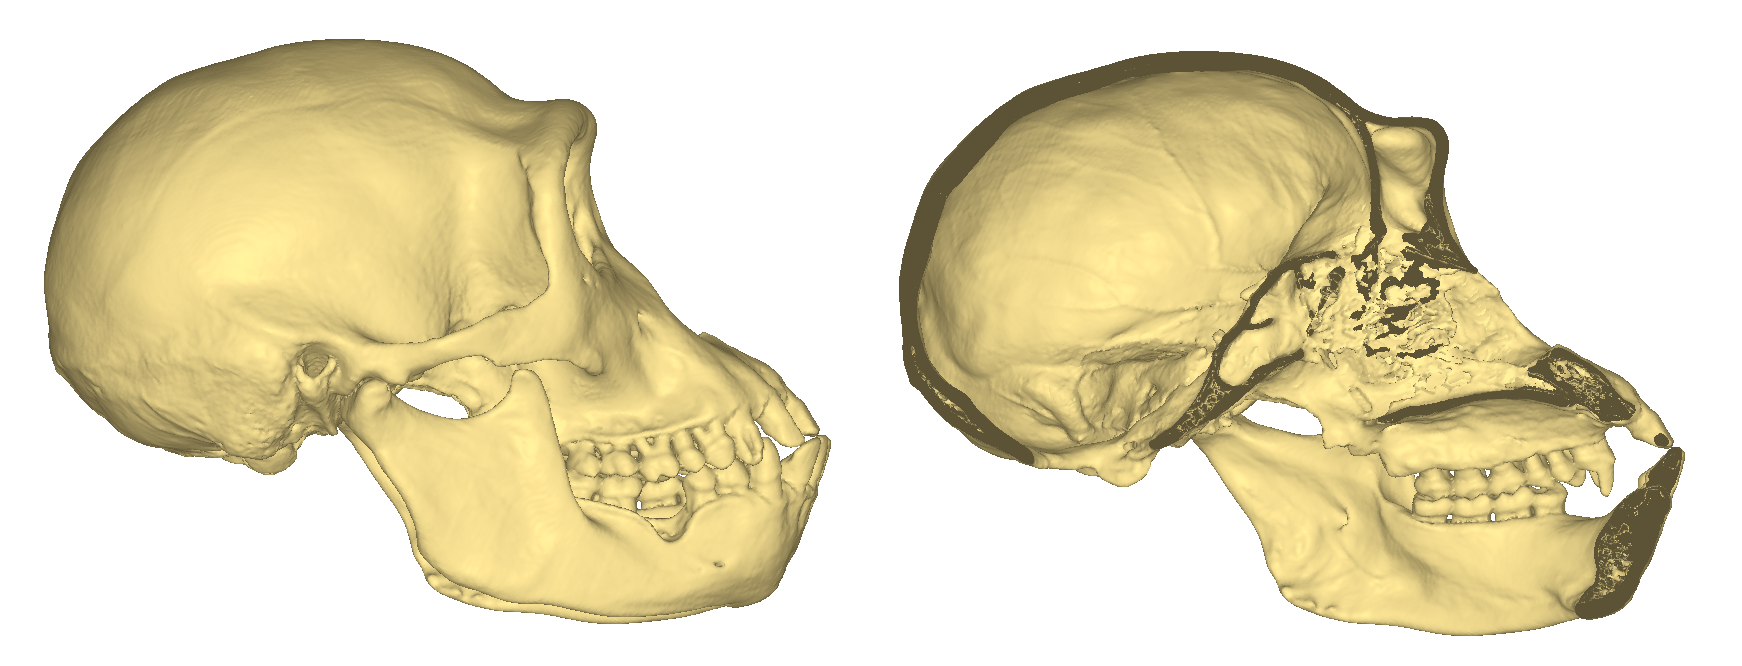
\includegraphics[scale=0.25]{images/Examples/Clipping_plane.png} 
	\caption{Left : cranium and mandible of the type specimen of \textit{Pan paniscus}(downloadable at http://www.metafro.be/primates/panpaniscustype ) rendered with the clipping plane placed at its original position. Right : the same skull viewed using a clipping plane placed at the position of the sagittal plane, revealing inner structures such as the endocranium cavity. Note that the position of the specimen was modified so that the sagittal plane of the skull passes  through the point (0,0,0) and is perpendicular to the vector (0,1,0).}
 
\end{figure}


\noindent
\begin{minipage}{0.55\textwidth}
\section{Camera}
\subsection{Camera options}


- Camera near, Camera far : define near and far clipping -
planes of the camera\\
- Azimuth, Elevation, Twist : camera rotation parameters\\
- Tx, Ty, Tz : camera translation in x, y and z\\

The buttons 
\includegraphics[scale=0.7]{images/pixmap/Clipping_plane_z0.png} and 
\includegraphics[scale=0.7]{images/pixmap/Clipping_plane_normal.png} which lie underneath the Tz control(and also underneath the clipping plane slider in the main window) permit to adjust / readjust the position of the clipping plane at predefined positions :\\

\end{minipage}  
 \begin{minipage}{0.45\textwidth}\centering
  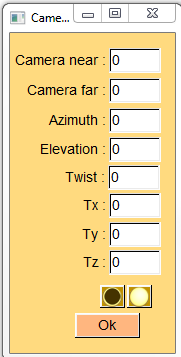
\includegraphics[scale=0.5]{images/Icons/camera_options.png}
 \captionof{figure}{Camera options window}

 \end{minipage} 
\noindent
- 
\includegraphics[scale=0.7]{images/pixmap/Clipping_plane_z0.png}: the clipping plane is placed at z = 0 (all objects having a z coordinate along z viewing axis smaller than 0 are hidden).\\
\noindent- 
\includegraphics[scale=0.7]{images/pixmap/Clipping_plane_normal.png}: the clipping plane is replaced at its original value : z= - camera.far / 2. This value permits to view objects having positive and negative coordinates along z viewing axis.

\subsection{Camera rotation centre at}\label{camera_centre_at}



Camera rotation centre can be set at the origin of the coordinate system (x=0, y=0, z=0) or at the location of one of the first 10 ``normal" landmarks.

\subsection{Set 100 pixels in mm}

\noindent
\begin{minipage}{0.55\textwidth}
Camera zoom can be modified in order to reach a desired display pixel size. This is useful to produce scaled images.

\end{minipage}  
 \begin{minipage}{0.45\textwidth}\centering
  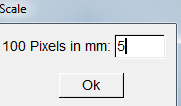
\includegraphics[scale=0.5]{images/Icons/100px_mm.png}
 \captionof{figure}{Scale window\\}

 \end{minipage} 
\noindent


\subsection{Reset camera}
You may use this option to reinitialize camera parameters.
\section{Object rendering options}

\noindent
\begin{minipage}{0.55\textwidth}



\subsection{Gouraud shading}
This is the default rendering mode. Object rendering is performed using vertices' normals.

\end{minipage}  
 \begin{minipage}{0.45\textwidth}\centering




 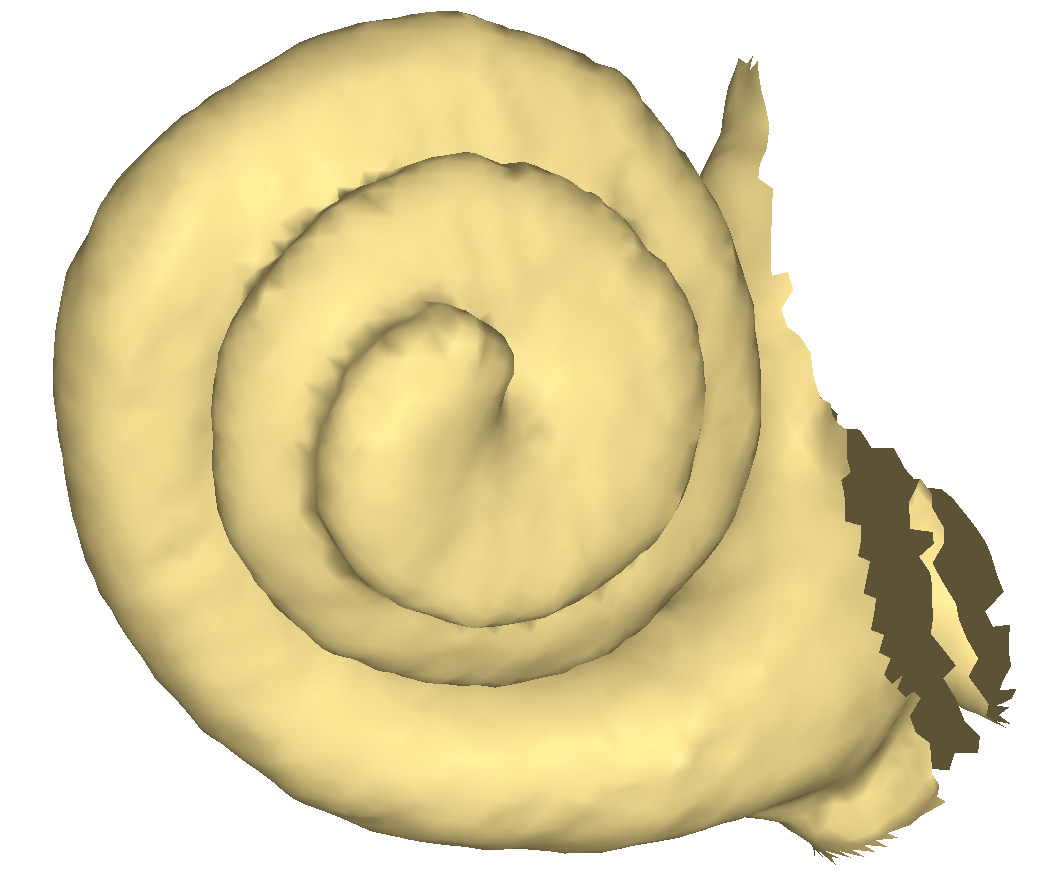
\includegraphics[scale=0.1]{images/Viewing_options/Normal_gouraud.png}
 \captionof{figure}{Gouraud shading}

 \end{minipage} 
\noindent


\noindent
\begin{minipage}{0.55\textwidth}

\subsection{Draw wireframe}
This option can be useful to inspect the structure of the surface.

\end{minipage}  
 \begin{minipage}{0.45\textwidth}\centering

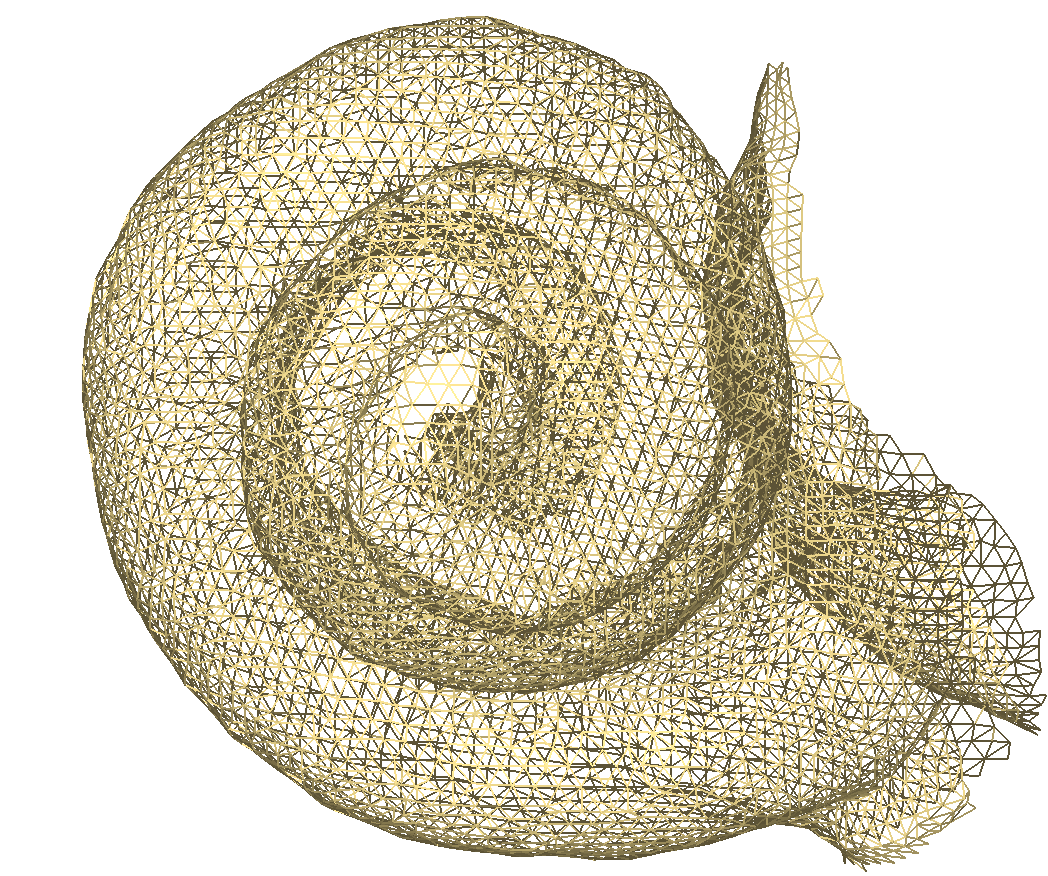
\includegraphics[scale=0.1]{images/Viewing_options/wireframe.png}
 \captionof{figure}{Example of wireframe rendering}

 \end{minipage} 
\noindent

\noindent
\begin{minipage}{0.55\textwidth}
\subsection{Sort vertices from back to front}\label{sort_back_front}
This option is (only) useful when working with transparent surfaces, in the case you want to display all surface inner structures. When active, whenever the camera of the
object is moved, vertices will be sorted in order to be displayed from back to front. This is the way transparency is achieved in OpenGL. As a consequence, rendering fluidity
becomes slow when working with heavy surfaces and/or a large number of objects. To change the transparency of an object, select an object, and reach ``Edit selected surfaces $\rightarrow$
Rendering modifications $\rightarrow$ Set alpha value".\\

Alternatively, in order to increase rendering fluidity, you may chose not to use the ``Sort vertices from back to front beware: slow rendering)" rendering option, but to sort episodically the vertices from back to front by pressing the button 
\includegraphics[scale=0.7]{images/pixmap/Sort_vertices01.png}.\\
Working with transparency is useful to observe inner structures and/or when digitizing landmarks
inside structures.

\end{minipage}  
 \begin{minipage}{0.45\textwidth}\centering

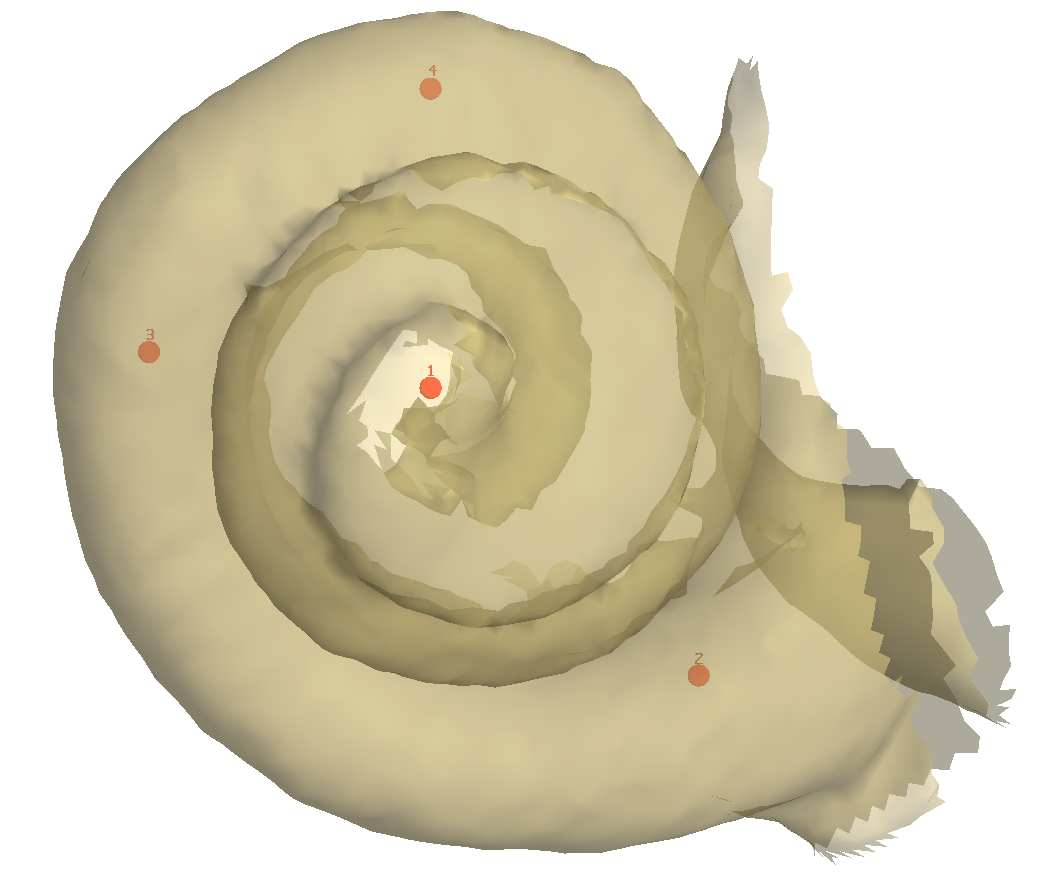
\includegraphics[scale=0.1]{images/Viewing_options/Sort_back_front.png}
 \captionof{figure}{Sort vertices from back to front.In this example, vertices are displayed from back to front. Four landmarks placed within this structure can be visualized.}

 \end{minipage} 
\noindent


\noindent
\begin{minipage}{0.55\textwidth}

\subsection{Sort vertices from front to back}\label{sort_front_back}
This option is (only) useful when working with transparent surfaces, and when you do not want to display too many inner structures. When active, whenever the camera of the object is moved, vertices will be sorted in order to be displayed from front to back. As a consequence, rendering fluidity becomes slow when working with heavy surfaces and/or a large number of objects. Alternatively, in order to increase rendering fluidity, you may chose not to use the ``Sort vertices from front to back (beware: slow rendering)" rendering option, but to sort
episodically the vertices from front to back by pressing the button 
\includegraphics[scale=0.7]{images/pixmap/Sort_vertices02.png}.

\end{minipage}  
 \begin{minipage}{0.45\textwidth}\centering

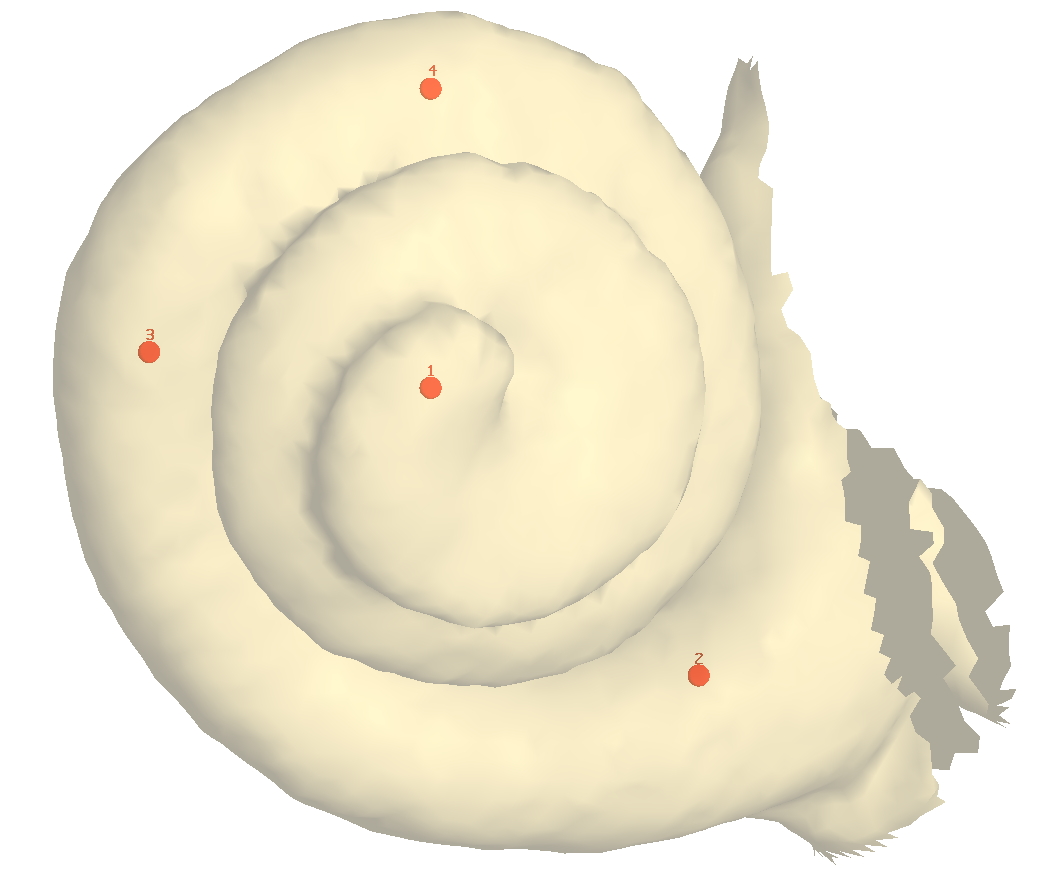
\includegraphics[scale=0.1]{images/Viewing_options/Sort_front_back.png}
 \captionof{figure}{Sort vertices from front to back.}

 \end{minipage} 
\noindent

\noindent
\begin{minipage}{0.55\textwidth}

\subsection{Flat triangles}
Using this option improves the perception of surface structure.

\end{minipage}  
 \begin{minipage}{0.45\textwidth}\centering
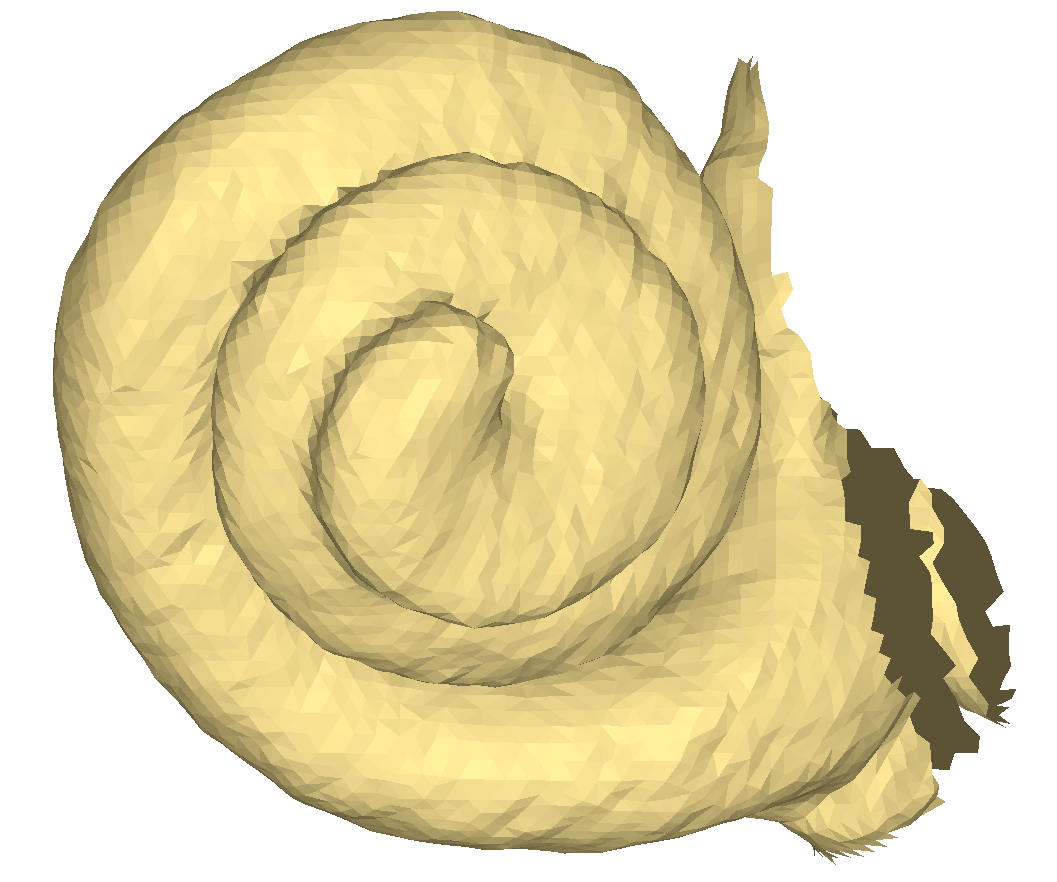
\includegraphics[scale=0.1]{images/Viewing_options/Triangles.png}
 \captionof{figure}{Example of flat triangle surface rendering}

 \end{minipage} 
\noindent

\noindent
\begin{minipage}{0.55\textwidth}

\subsection{Wireframe and flat triangles}
Using this option further improves the perception of surface structure.

\end{minipage}  
 \begin{minipage}{0.45\textwidth}\centering


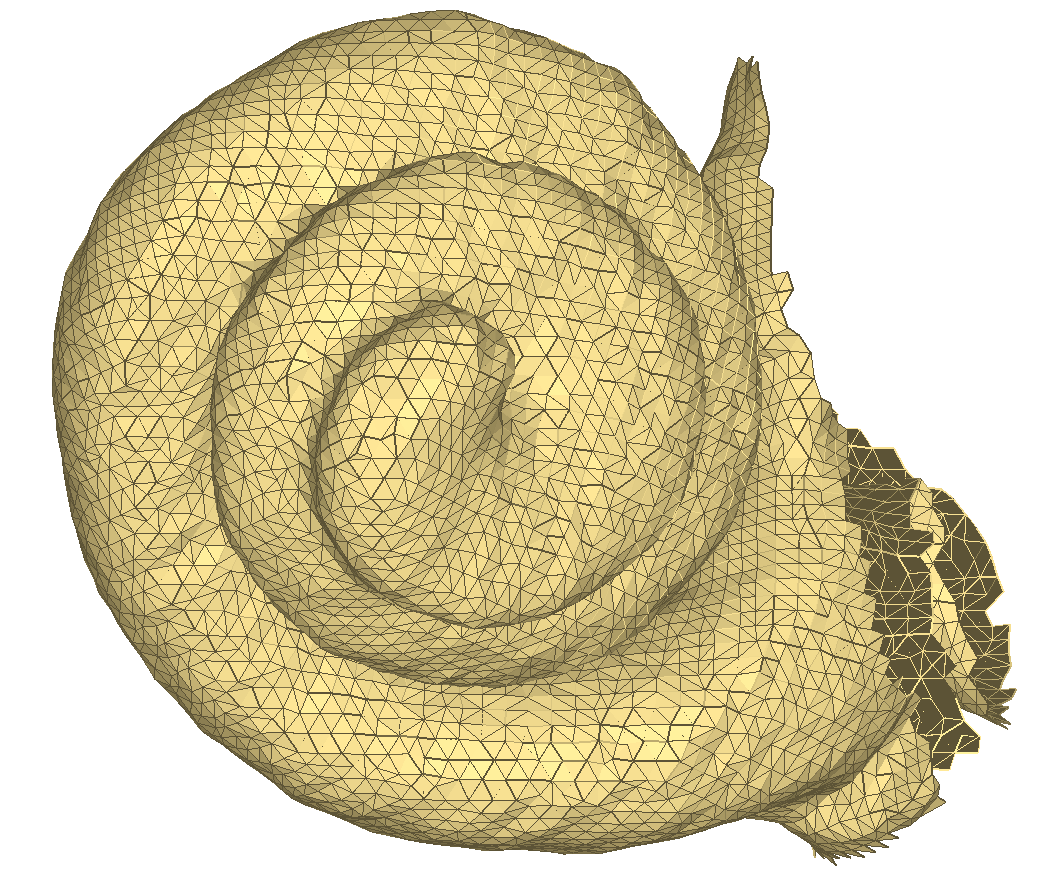
\includegraphics[scale=0.1]{images/Viewing_options/Triangle_flat_triangles.png}
 \captionof{figure}{Example of flat triangle + wireframe surface rendering}

 \end{minipage} 
\noindent




\noindent
\begin{minipage}{0.55\textwidth}

\subsection{Backface culling}
Surface's back faces are hidden when using this option.
\end{minipage}  
 \begin{minipage}{0.45\textwidth}\centering

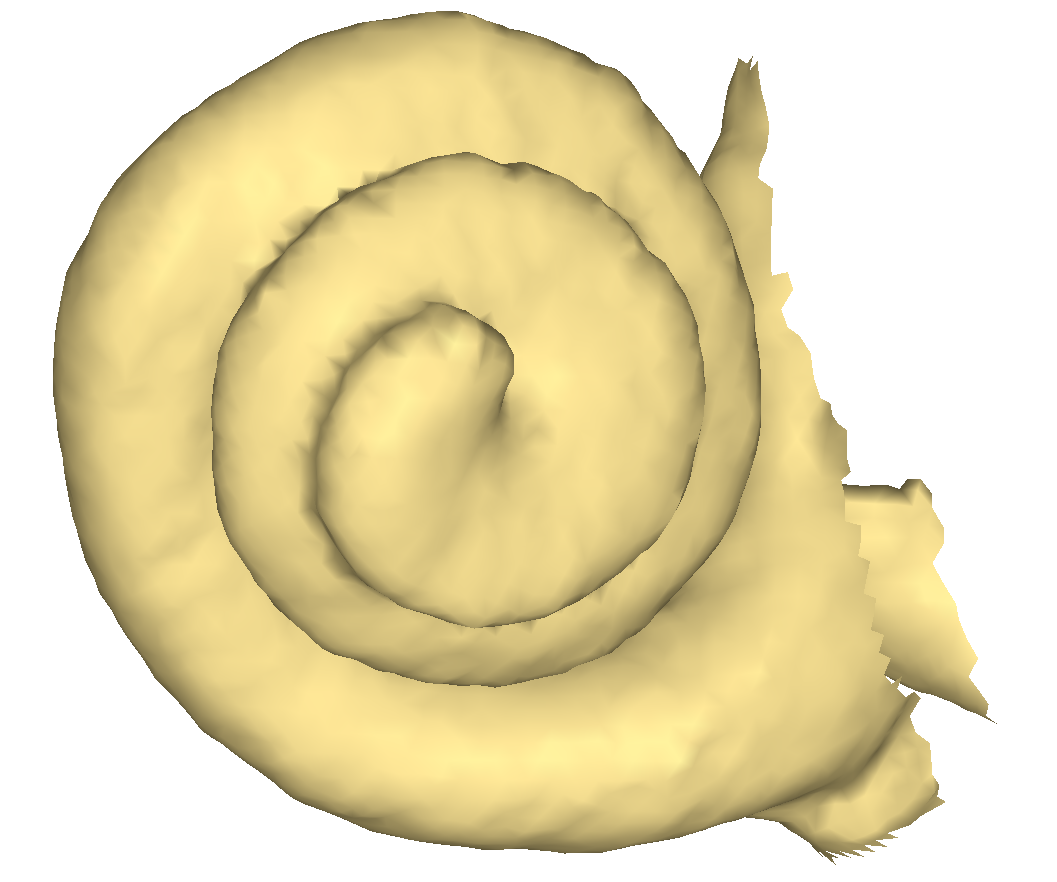
\includegraphics[scale=0.1]{images/Viewing_options/Backface_culling.png}
 \captionof{figure}{Backface culling rendering}

 \end{minipage} 
\noindent




\subsection{Display vertices ids}
For surface inspection purposes, you may sometimes need to visualize vertices ids. Note : this option affects rendering fluidity even when using relatively light surfaces.

\subsection{Display triangle ids}
For surface inspection purposes, you may sometimes need to visualize triangle ids.\\
Note : this option affects rendering fluidity even when using relatively light surfaces.\\



\noindent
\begin{minipage}{0.45\textwidth}\centering
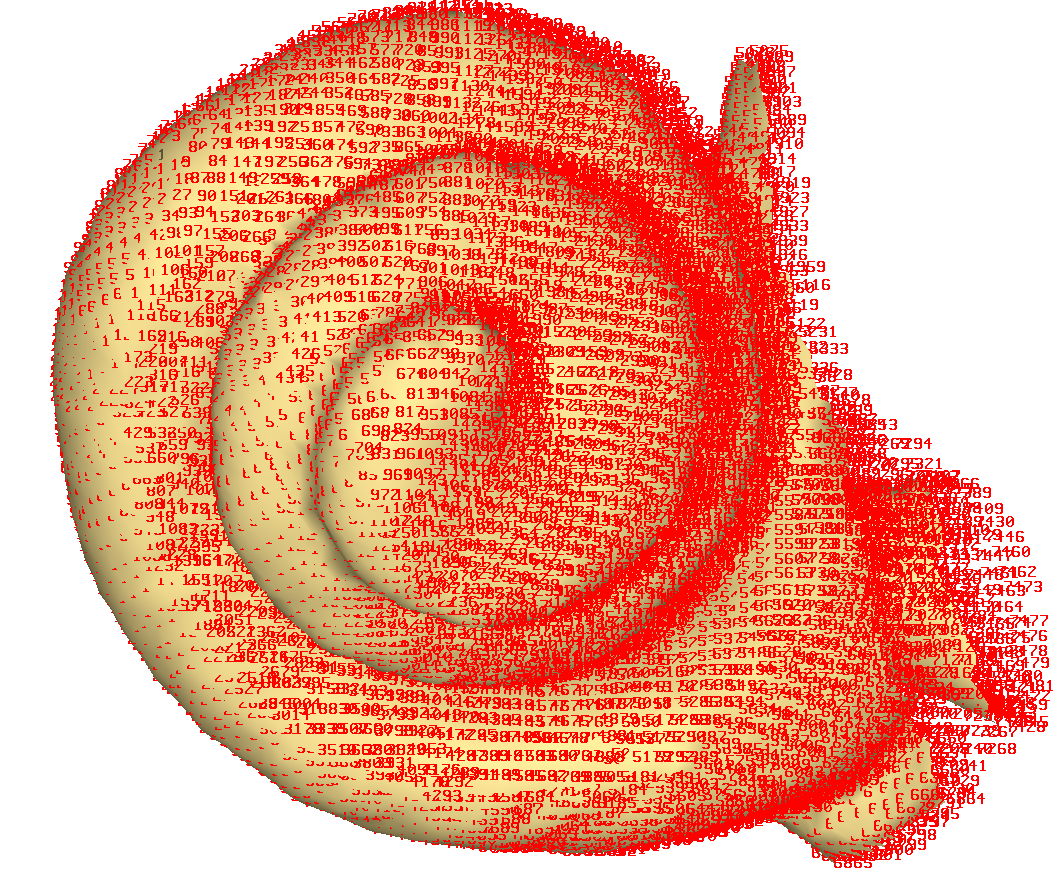
\includegraphics[scale=0.1]{images/Viewing_options/Vertices_ids.png}
 \captionof{figure}{Gouraud shading + vertices ids rendering}

\end{minipage}  
 \begin{minipage}{0.45\textwidth}\centering
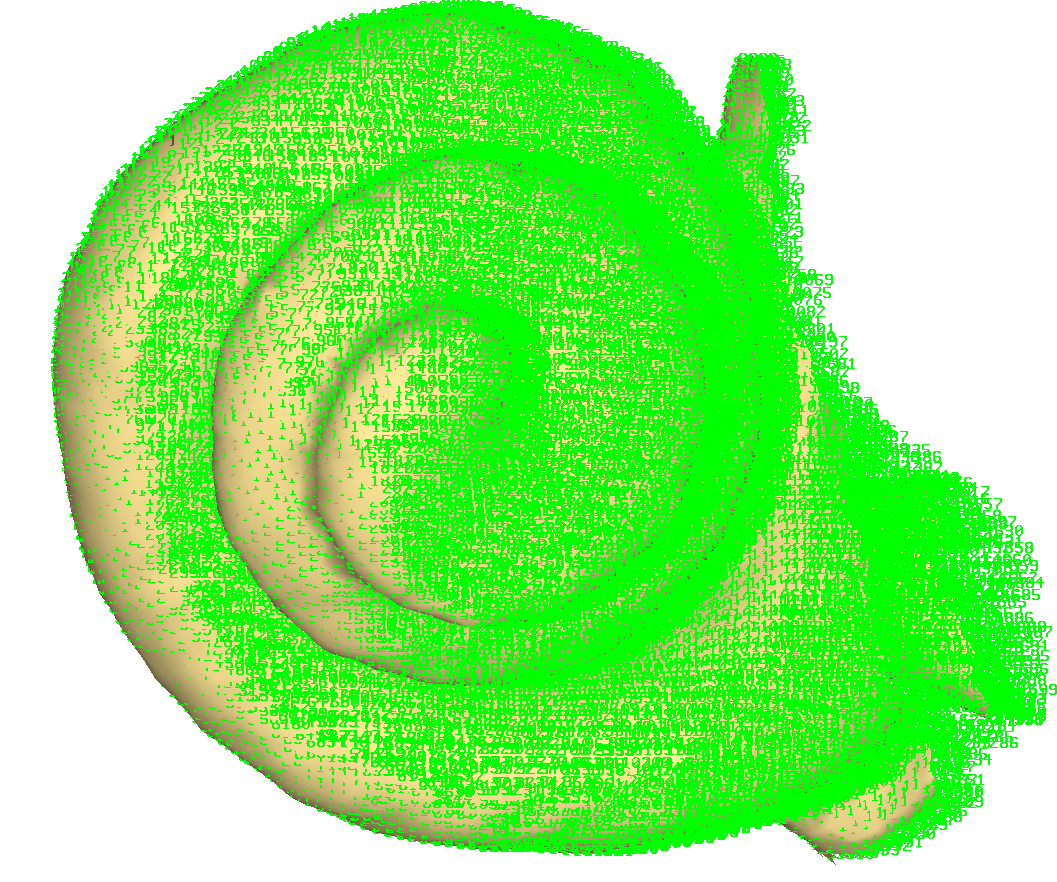
\includegraphics[scale=0.1]{images/Viewing_options/Triangle_ids.png}
 \captionof{figure}{Gouraud shading + triangle ids rendering}

 \end{minipage} 
\noindent





\section{Grid size}


\noindent
\begin{minipage}{0.55\textwidth}
Grid rendering can be edited to reach the desired size/square
\end{minipage}  
 \begin{minipage}{0.45\textwidth}\centering
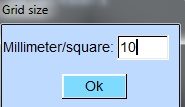
\includegraphics[scale=0.5]{images/Viewing_options/Grid_size.png}
 \captionof{figure}{Grid size window}

 \end{minipage} 
\noindent





\section{Landmark and flag rendering options}
The landmark and flag options window (see Fig. \ref{landmarks_flags_options}) contains the following sections:

\subsection{Landmarks rendering}
``Normal" and ``Target" landmarks can be drawn as spheres or as needles. Landmark display size can be chosen to be adjusted automatically (default behaviour) or edited manually (when you feel that the automatic adjustment does not meet your needs) also edited manually in this section.



\subsection{Flags settings}
Flag length and colour settings can be defined in thissubsection. Once placed on a surface and selected, the colour, the length and the label of the flag can be changed by pressing

\includegraphics[scale=0.7]{images/pixmap/Flag02.png}.


\begin{figure}
  \centering  
 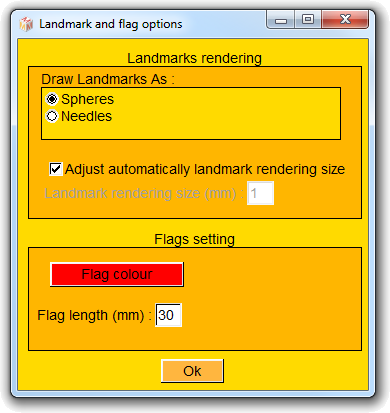
\includegraphics[scale=0.5]{images/Viewing_options/Landmark_options.png}
 \captionof{figure}{Landmark and flag options window.}
\label{landmarks_flags_options}
\end{figure}

\section{Display landmark numbers}
``Normal" and ``target" landmark numbers are displayed by default. For illustration purposes, you may sometimes need to hide landmark numbers.

\section{Draw curves}
Activate/deactivate this option to draw/hide 3D Bezier curves passing through ``normal" landmarks. See the tutorial ``working with curves" for further details regarding curve digitization with ISEMeshTools.

\section{Orientation labels}


\noindent
\begin{minipage}{0.55\textwidth}
The labels associated to the 6 orientation axes can be modified using this window. This will affect the coordinate system orientation helper displayed on the bottom left area of the 3D
window.

\end{minipage}  
 \begin{minipage}{0.45\textwidth}\centering
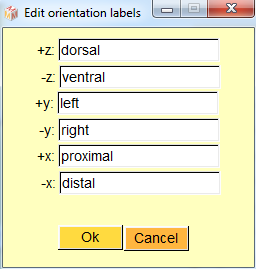
\includegraphics[scale=0.5]{images/Viewing_options/Object_labels.png}
 \captionof{figure}{Edit orientation labels window}

 \end{minipage} 
\noindent



\section{VBO activate (GPU acceleration)}
By default, ISE-MeshTools does not use the graphic card to display 3D objects, which slows down dramatically the rendering speed of heavy 3D meshes and that of tagged meshes. However, we have chosen not to activate the ``VBO" rendering option by default, as we have experienced that it causes ISE-MeshTools to crash on old computers or on some others which have not up to date graphic card drivers. By activating the graphic card acceleration option (VBO activate), you will probably find out that ISE-MeshTools is much more fluid to work with.\\ This feature was implemented by Cécile Peladan.

